\begin{figure}[h]
	\centering
    \begin{tikzpicture}
    \node[inner sep=0pt] (pic) at (0,0)
    {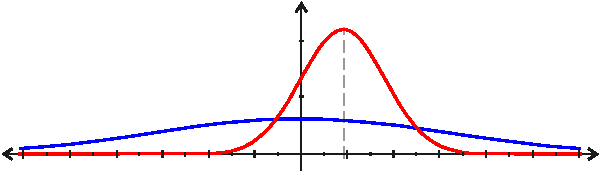
\includegraphics[width=15.5cm]{pictures/picture_2_5.pdf}};
    \draw [color=red](3,0.2) node[anchor=north west] {$ \pi ( \mu | x ) $};
    \draw [color=blue](-5.2,-0.5) node[anchor=north west] {$ \pi (\mu) $};
    \draw [color=gray](0.6,-1.8) node[anchor=north west] {$ ^{10}/_{11} $};
    \end{tikzpicture}
    \caption{Vykreslení apriorní hustoty a aposteriorní hustoty pravděpodobnosti.}
\end{figure}